\section{Présentation du sujet} % Pas de numérotation
\addcontentsline{toc}{section}{Présentation du sujet} % Ajout dans la table des matières

\subsection{Un rapide résumé}
Le jeu que nous nous sommes proposés de réaliser est un beat’em’all et tower defense s’inspirant du jeu BoxHead. Le
principe général est de survivre sur une carte à plusieurs vagues successives d’ennemis. Pour se faire,
le joueur incarne un personnage en vue à la troisième personne qui peut se déplacer, attaquer à distance avec des sorts 
et construire des tours.

\begin{figure}[!ht]
    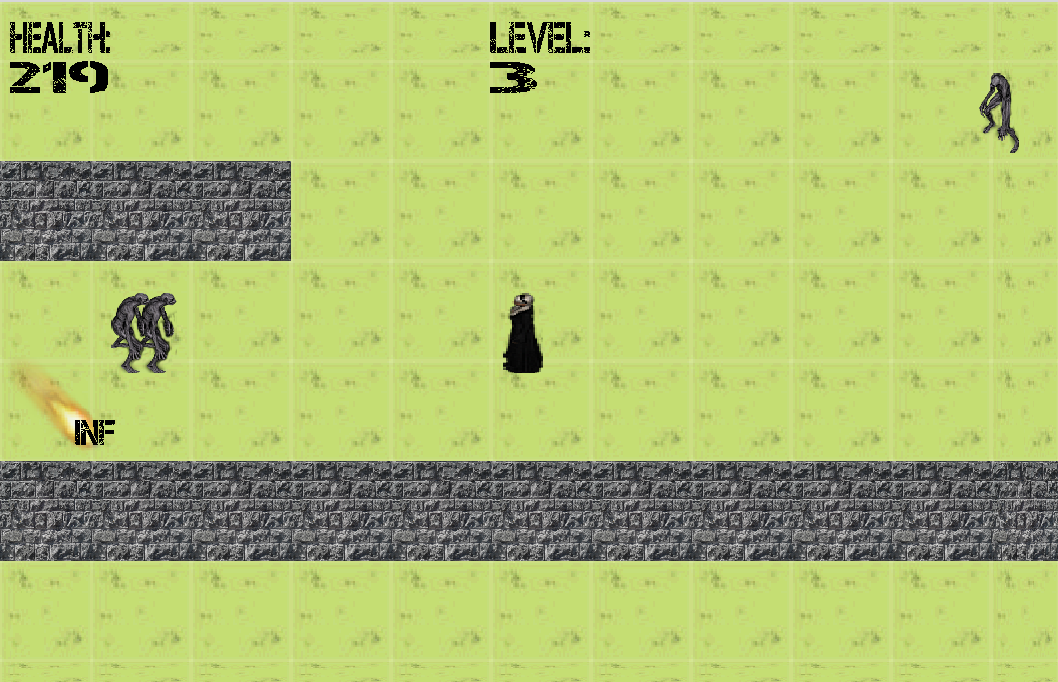
\includegraphics[width=0.5\textwidth]{./images/snapshot1.png}
    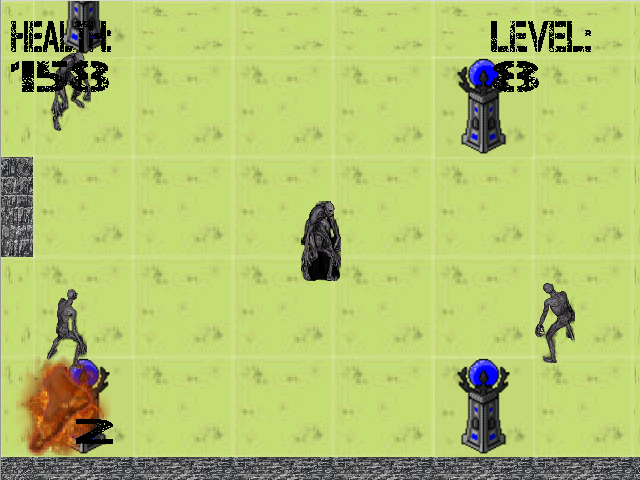
\includegraphics[width=0.5\textwidth]{./images/snapshot2.png}
    \caption{Snapshots}
\end{figure}

Les touches par défaut sont :
\begin{itemize}
\item[•][Flèches directionnelles] pour les déplacements
\item[•][Espace] pour lancer un sort
\item[•][a] [z] [e] pour naviguer entre les sorts
\end{itemize}
\subsection{Une licence pour les protéger tous}

Le logiciel et l'ensemble des sources sont sous licence CC BY-NC-SA 3.0 FR. Le partage et l'adaptation du logiciel sont permises à condition de ne pas l'utiliser
commercialement, d'indiquer les changements effectués, de référencer l’œuvre originale et 
de conserver la même licence.

\subsection{Le cahier des charges}

Afin de gérer au mieux le projet, avons établi un cahier des charges minimal ainsi qu'un cahier des charges facultatif dont les options ont été implémentées en fonction de leur difficulté et du temps imparti. \\
Cahier des charges minimal :
\begin{itemize}
\item Lancement d’une partie sur une carte unique
\item Interaction avec le clavier pour se déplacer et attaquer
\item Gestion de l’interaction avec l’environnement (collision, ...)
\item Création d’un dispositif de défense
\item Menu d’accueil
\end{itemize}
Fonctionnalités optionnelles :
\begin{itemize}
\item Capacités spéciales à usage limité
\item Difficulté croissante des ennemis dans le temps (ennemis plus rapides, plus résistants, ...)
\item Mode coopératif/deathmatch à deux en réseau ou sur le même clavier
\item Choix de la difficulté générale
\item Éditeur et choix de carte
\end{itemize}